\chapter{Transport domain}

\section{Automated planning}

Planning is usually defined as the reasoning side of acting -- an abstract deliberation
process that chooses and organizes actions by anticipating their outcomes. \cite[Section~1.1]{Ghallab2004}
It seems only natural that we want to have computers to do this strenuous activity for us.
Automated planning is an attempt at just that -- it is an area of Artificial Intelligence (AI) that
studies the planning process computationally. \cite[Section~1.1]{Ghallab2004}

\TODO{Define domain and problem, planner?}

Unfortunately, the specific situations in which we want to use automated planning are very diverse --
from devising a sequence of actions to shut down a nuclear power plant to planning the robotic arm
movements in an assembly line or devising the complex motor activations for space aircraft positioning.
Due to this, people are often interested in domain-independent planning, where the planner gets information
about both the domain and the specific problem and attempts to devise a plan using only the provided knowledge
and its previously built-in processes. \cite[Section~1.3]{Ghallab2004}

On the other hand, domain-specific planning, where domain knowledge has been built into the planner,
has obvious advantages when solving problems in that domain -- all the while being useless on problems of other
domains. \cite[Section~1.3]{Ghallab2004}

\subsection{Planning model}

As a basis for the later-defined representation of planning, we first define
a conceptual model similar to the restricted model in \cite[Section~1.4, Section~1.5]{Ghallab2004}.

\begin{defn}[State-transition system]\label{defn:state-transition-sys}
A (restricted) state-transition system is a 3-tuple $\Sigma = (S, A, \gamma)$, where:
\begin{itemize}
\item $S = \{s_1, s_2, \ldots\}$ is a finite and fully observable set of states,
\item $A = \{\noop, a_1, a_2, \ldots\}$ is a finite set of actions;
\item $\gamma: S \times A \to S \cup \{\emptyset\}$ is a state-transition function,
where $\forall s \in S : \gamma(s, \noop) = s$,
and $\forall s \in S\,\exists a \in A : \gamma(s, a) \neq \emptyset$; and
\item $\Sigma$ is static and offline,
it only changes when an action is applied to it and does not change while planning.
\end{itemize}
In the basic version, all actions have no duration.
\end{defn}

\noindent \TODO{define goals and mention that planning domains correspond to state-transition systems}

\begin{defn}[Planning problem]\label{defn:planning-problem}\cite[Part~I]{Ghallab2004}
A planning problem is a 5-tuple $\mathcal{P} = (S, A, \gamma, s_0, g)$, where:
\begin{itemize}
\item $(S, A, \gamma)$ is a state-transition system;
\item $s_0 \in S$ is an initial state; and
\item $g \subseteq S$ is a set of goal states.
\end{itemize}
\end{defn}

\noindent For notation purposes, we define $[k] := \{1, 2, \ldots, k\}$ for all $k \in \N$

\begin{defn}[Plan]\label{defn:plan}\cite[Section~1.5]{Ghallab2004}
For a planning problem $\mathcal{P} = (S, A, \gamma, s_0, g)$,
a plan is a finite ($k \in \N$) sequence of actions $(a_1, a_2, \ldots, a_k)$ where
$\forall i \in [k] : a_i \in A$ such that
$\forall i \in [k] : \gamma(s_{i-1}, a_i) = s_i$ and $s_k \in g$.
\end{defn}

\noindent A basic planning model (see figure \ref{fig:planning-model}) consists of three components:

\begin{itemize}
\item A \textit{state-transition system} $\Sigma$ that evolves by its state-transition function using the actions
it receives.
\item A \textit{controller} -- given an input state $s \in S$ provides an action $a \in A$ as output according
to a plan.
\item A \textit{planner} -- uses a description of $\Sigma$ to synthesize a plan for the controller
to execute in order to achieve the objective.
\end{itemize}

\begin{figure}[htb]
\begin{center}
\includegraphics[width=0.7\textwidth]{../img/planning_model}
\end{center}
\caption{Typical planning model for offline planning. Adapted from \cite[Figure 1.3]{Ghallab2004}.}
\label{fig:planning-model}
\end{figure}

\subsection{Classical planning}\label{classical-planning}

Although the previously defined restricted state-transition system is a simplification of real-world
problems, it is a useful one. 
This simplification has historically been studied as classical planning.
There are several theoretical domain-independent representations
of planning problems in classical planning: \cite[Chapter 2]{Ghallab2004}

\TODO{Move to sub sub sections* for clarity}

\begin{itemize}

\item \textbf{Set-theoretic representation}: both the planning domain and problem are represented with the notion
of proposition symbols $L = \{p_1, p_2, \ldots\}$. Each state is defined as a subset of $L$, each action
is a 3-tuple of subsets of $L$: $a = (\precond(a), \effects^-(a), \effects^+(a))$ -- the preconditions and
the negative and positive effects of $a \in A$. $S$ is closed under the application of effects
for each $a \in A$. The state-transition function is $\gamma(s, a) = (s - \effects^-(a)) \,\cup\,
\effects^+(a)$ if $a$ is applicable to $s$,
otherwise $\gamma(s, a)$ is undefined. Goal states are defined inductively using the goal propositions
$g \subseteq L$ as $S_g = \{s \in S \,|\, g \subseteq L\}$.
 
\item \textbf{Classical representation}:
generalizes the set-theoretic representation using first-order logic, without functions.
States are sets of ground atoms of a first-order language.
Actions are ground instances of \textit{planning operators}
-- triples $o = (\name(o), \precond(o), \effects(o))$,
where $\name(o)$ is a syntactic expression of the given operator;
$\precond(o)$ and $\effects(o)$ are sets of literals (atoms and their negations),
similar to the set-theoretic case.
The definition of the state-transition function is the same.
Goal states are defined as the set of states that satisfy $g$, the goal, where $g$ is any set
of ground literals.

\TODO{Relation of $\Sigma$ to $\mathcal{P}$, Soundness, extensions?}

\item \textbf{State-variable representation}: substitutes the use of relations of the two previous representations for functions, using the concept of state variables. State-variable functions are \TODO{def}.

\end{itemize}

Both the set-theoretic and the classical representations follow the \textit{Closed world assumption} -- that any atom/predicate not present in the state does not hold in the state.

\subsection{Neoclassical planning}



\subsection{Temporal planning}



\section{Transport domain description}

Transport is a planning domain designed for
the International Planning
Competition\footnote{\url{http://www.icaps-conference.org/index.php/Main/Competitions}}
(IPC), which is part of the International Conference on Automated Planning and
Scheduling\footnote{\url{http://www.icaps-conference.org/index.php/Main/HomePage}} (ICAPS).

Originally, Transport appeared at 
IPC-6\footnote{\url{http://icaps-conference.org/ipc2008/deterministic/Domains.html}} which took place in 2008.
Since then, it has been used in two IPCs,
specifically IPC-7\footnote{\url{http://www.plg.inf.uc3m.es/ipc2011-deterministic/}} in 2011
and IPC-8\footnote{\url{https://helios.hud.ac.uk/scommv/IPC-14/}} in 2014.

There are a few basic formulations of the Transport domain family (i.e.~``similar Transport domains'').

\subsection{Common traits of Transport domains}

Transport is a logistics domain -- vehicles drive around on a (generally asymmetric) positively-weighted oriented graph, picking up and dropping packages along the way.
All vehicles have limited capacities (the sum of package sizes they can carry).
Picking up or dropping a package costs 1 unit. The cost of driving along a road is equal to the edge weight
(in other words, the road length).
The general goal is to minimize the total cost
while delivering all packages to their destination.

\subsection{Transport STRIPS description}\label{transport-strips}

STRIPS, the Stanford Research Institute Problem Solver\cite{Fikes1971},
was a planner proposed in the 1970's by Fikes and Nilsson.
The influence of STRIPS was, however, not due to the planner,
but the language used to describe its inputs -- the planning operators and goals.
That is why we sometimes refer to classical planning (section \ref{classical-planning})
as STRIPS planning. For the purposes of this text, we will use these terms interchangeably.

In the STRIPS variant of the Transport domain,
all packages have a size of 1 and vehicles can drive around infinitely,
only incurring the cost of the travel. This being a classical STRIPS domain,
it does not assume time in any sense,
so actions have no duration and are applied one after the other, sequentially.

This formulation contains three basic planning operators:

\begin{itemize}
\item \verb+drive+: where a vehicle drives to an adjacent location
along a road that is connected to its current location;
\item \verb+pick-up+: where a vehicle that is stationary at a location picks up a co-located package; and
\item \verb+drop+: where a stationary vehicle drops a package off at its location.
\end{itemize}

In all the datasets, this domain variant is denoted as \textit{Transport sequential}
or \textit{transport-strips} and we will alternate between these terms in this text.

\subsection{Transport Numeric description}\label{transport-numeric}

The numeric variant adds the concept of fuel on top of the STRIPS variant.
All roads have an additional cost, called \verb+fuel-demand+, which is
subtracted from a vehicle's \verb+fuel-left+ value if it chooses to drive along that road.
Additionally, all vehicles have a maximum fuel capacity \verb+fuel-max+,
which they regain upon being the target of a \verb+refuel+ action. This action can only
be executed at a location that is marked as having a petrol station. Petrol stations
are static with respect to a given planning problem instance.

This variant is usually denoted as \textit{Transport netbenefit} or \textit{transport-numeric}

\TODO{mention weird goal requirements of netben problems?}

\subsection{Transport Temporal description}\label{transport-temporal}

The temporal Transport domain is usually denoted as \textit{Transport temporal} or, confusingly,
also \textit{transport-numeric}. A major difference with respect to the numeric variant is
the addition of time. All actions now have a duration (\verb+pick-up+ and \verb+drop+ both have a
duration of 1, \verb+refuel+ has a duration of 10, and the duration of \verb+drive+ is
equal to the length of the road we are driving along). Furthermore, packages can now have any integral size.

The addition of time poses numerous technical complications when formalizing this variant
-- its PDDL formulation significantly differs the two previous ones, but only in technical details.
One important technicality is that a vehicle cannot pick up or drop packages concurrently -- it always handles packages one at a time. Also, vehicles cannot do other actions during driving to another location (they are essentially placed ``off the graph'' for the duration of driving).

The overall goal remains largely the same (deliver packages to their destinations), but we no longer optimize the total cost. Instead, we now minimize the total duration of a plan (in practice, this translates to minimizing
maximum end time over all actions).



\section{Transport domain formulation}

\TODO{intro}

\subsection{Transport's classical representation}

\TODO{Remove me?}

We are now able to show the sequential Transport domain in one of the representations
previously defined, namely,
the classical representation (figure \ref{code:classical-strips}).

\TODO{Expand description}

\TODO{Add total-cost to the code below?}

\begin{figure}[htb]
\begin{code}
drive(v, l1, l2)
  ;; vehicle v moves from location l1 to an adjacent location l2
  precond: at(v, l1), road(l1, l2)
  effects: not at(v, l1), at(v, l2)

pick-up(v, l, p, s1, s2)
  ;; vehicle v picks up package p at location l,
  ;; decreasing its capacity from s2 to s1
  precond: at(v, l), at(p, l), capacity-predecessor(s1, s2),
           capacity(v, s2)
  effects: not at(p, l), in(p, v), capacity(v, s1),
           not capacity(v, s2)
  
drop(v, l, p, s1, s2)
  ;; vehicle v drops package p at location l,
  ;; increasing its capacity from s1 to s2
  precond: at(v, l), in(p, v), capacity-predecessor(s1, s2),
           capacity(v, s1)
  effects: not in(p, v), at(p, l), capacity(v, s2),
           not capacity(v, s1)
\end{code}
\caption{Classical formulation of \texttt{transport-strips}.}
\label{code:classical-strips}
\end{figure}

The numeric variant adds the \verb+refuel+ operator and changes \verb+drive+ (see figure \ref{code:classical-numeric}).

\begin{figure}[htb]
\begin{code}
drive(v, l1, l2)
  ;; vehicle v moves from location l1 to an adjacent location l2
  precond: at(v, l1), road(l1, l2), fuel-left(v) >= fuel-demand(l1, l2)
  effects: not at(v, l1), at(v, l2),
           decrease(fuel-left(v),  fuel-demand(l1, l2))
  
refuel(v, l)
  ;; vehicle v is refueled to the maximum at location l
  precond: at(v, l), has-petrol-station(l)
  effects: assign(fuel-left(v), fuel-max(v))
\end{code}
\caption{Classical formulation of \texttt{transport-numeric}'s differences.}
\label{code:classical-numeric}
\end{figure}

\subsection{Temporal Transport's classical representation}

\TODO{code + explanation}

\subsection{Transport's state-variable representation}

We are now able to show the sequential Transport domain
in one of the representations previously defined, namely,
the state-variable representation (figure \ref{code:statevar-strips}).

\TODO{expand description}

\TODO{Add total-cost to the code below?}

\begin{figure}[htb]
\begin{code}
drive(v, l1, l2)
  ;; vehicle v moves from location l1 to an adjacent location l2
  precond: at(v) = l1, road(l1, l2)
  effects: at(v) <- l2

pick-up(v, l, p, s1, s2)
  ;; vehicle v picks up package p at location l,
  ;; decreasing its capacity from s2 to s1
  precond: at(v) = l, at(p) = l, capacity-predecessor(s1, s2),
           capacity(v) = s2
  effects: at(p) <- nil, in(p) <- v, capacity(v) <- s1
  
drop(v, l, p, s1, s2)
  ;; vehicle v drops package p at location l,
  ;; increasing its capacity from s1 to s2
  precond: at(v) = l, in(p) = v, capacity-predecessor(s1, s2),
           capacity(v) = s1
  effects: in(p) <- nil, at(p) <- l, capacity(v) <- s2
\end{code}
\caption{State-variable formulation of \texttt{transport-strips}.}
\label{code:statevar-strips}
\end{figure}

The numeric variant adds the \verb+refuel+ operator and changes \verb+drive+ (figure \ref{code:statevar-numeric}).

\begin{figure}[htb]
\begin{code}
drive(v, l1, l2)
  ;; vehicle v moves from location l1 to an adjacent location l2
  precond: at(v) = l1, road(l1, l2), fuel-left(v) >= fuel-demand(l1,l2)
  effects: at(v) <- l2, fuel-left(v) <-  fuel-demand(l1, l2)
  
refuel(v, l)
  ;; vehicle v is refueled to the maximum at location l
  precond: at(v) = l, has-petrol-station(l)
  effects: fuel-left(v) <- fuel-max(v)
\end{code}
\caption{State-variable formulation of \texttt{transport-numeric}'s differences.}
\label{code:statevar-numeric}
\end{figure}

\subsection{PDDL}

Originally proposed by McDermott et al. in 1998 for the 1$^{\mathrm{st}}$ International Planning
Competition\footnote{http://ipc98.icaps-conference.org/} (IPC),
the Planning Domain Definition Language\cite{McDermott1998} (PDDL) has become
a de facto standard language for modelling planning domains and problems,
continually evolving to the needs of the
research community and the needs of the IPC itself in the future years.

PDDL was inspired by the language used to describe STRIPS\cite{Fikes1971}
and the numerous languages that sparked from it.
It has a Lisp-like\footnote{\url{https://en.wikipedia.org/wiki/Lisp_(programming_language)}}
declarative syntax and is very extensible.
Not many planners support PDDL in its entirety -- they usually support 
several ``feature subsets'', called \textit{requirements}.
Over time, PDDL has evolved from the originally proposed version 1.2
to the now standard version 3.1. Several extensions and successors were proposed,
like Multi-Agent PDDL\comment{\footnote{\url{http://agents.fel.cvut.cz/codmap/}}}
(MA-PDDL) and
Probabilistic PDDL\comment{\footnote{\url{http://www.tempastic.org/papers/CMU-CS-04-167.pdf}}}
(PPDDL).

All formulations of the Transport domain use the basic PDDL version, with the requirement \verb+typing+.
The STRIPS variant additionally needs \verb+action-costs+, while the numeric variant
requires \verb+numeric-fluents+ and \verb+goal-utilities+.
The temporal domain is similar in requirements to the numeric one, except for
substituting \verb+goal-utilities+ for \verb+durative-actions+.
One problem with the diversity of these domain formulations is that rarely does
a single planner support the union of all these requirements.
We show the capabilities of individual studied planners
later on, in table \ref{tab:plannner-requirements-comparison}.

For reference, we show the PDDL representation of the sequential variant of
the Transport domain in figure \ref{code:pddl-strips}.

\begin{figure}[htb]
\begin{code}
(define (domain transport)
  (:requirements :typing :action-costs)
  (:types
        location target locatable - object
        vehicle package - locatable
        capacity-number - object)
  (:predicates 
     (road ?l1 ?l2 - location)
     (at ?x - locatable ?v - location)
     (in ?x - package ?v - vehicle)
     (capacity ?v - vehicle ?s1 - capacity-number)
     (capacity-predecessor ?s1 ?s2 - capacity-number))
  (:functions
     (road-length ?l1 ?l2 - location) - number
     (total-cost) - number)
     
  (:action drive
    :parameters (?v - vehicle ?l1 ?l2 - location)
    :precondition (and (at ?v ?l1) (road ?l1 ?l2))
    :effect (and (not (at ?v ?l1)) (at ?v ?l2)
        (increase (total-cost) (road-length ?l1 ?l2))))
        
 (:action pick-up
    :parameters (?v - vehicle ?l - location ?p - package
                 ?s1 ?s2 - capacity-number)
    :precondition (and (at ?v ?l) (at ?p ?l)
        (capacity-predecessor ?s1 ?s2) (capacity ?v ?s2))
    :effect (and (not (at ?p ?l)) (in ?p ?v) (capacity ?v ?s1)
        (not (capacity ?v ?s2)) (increase (total-cost) 1)))
        
  (:action drop
    :parameters (?v - vehicle ?l - location ?p - package
                 ?s1 ?s2 - capacity-number)
    :precondition (and (at ?v ?l) (in ?p ?v)
        (capacity-predecessor ?s1 ?s2) (capacity ?v ?s1))
    :effect (and (not (in ?p ?v)) (at ?p ?l) (capacity ?v ?s2)
        (not (capacity ?v ?s1)) (increase (total-cost) 1))))
\end{code}
\caption{PDDL formulation of \texttt{transport-strips}.}
\label{code:pddl-strips}
\end{figure}





\section{The Vehicle Routing Problem}

\TODO{mention Dantzig} \cite{Dantzig1959}

\TODO{mention Braekers} \cite{Braekers2016}

\TODO{mention Montoya} \cite{Montoya2015}

\TODO{mention Neo} \cite{NeoVrp}

\subsection{Constraint Satisfaction Problems}

\subsection{Problem formulation}

\subsection{Comparison to the Transport domain formulation}

\subsection{Formulating the sequential Transport domain as a VRP problem}

\TODO{Ghallab 8.3}
